\section{Setting, threat model and estimands}\label{sec:setting}
\subsection{Releases, adversary and success event}
Let $U$ be a finite population of units and $\theta$ a candidate release mechanism, such as a cell-count floor. A programme publishes releases $D_{\theta,1},\ldots,D_{\theta,V}$, one per vintage, each covering the units present at that vintage. A \emph{scenario} $a$ names an attacker, a harm, a subgroup and the set of vintages the attacker holds; a scenario that holds more than one vintage is a pooled attack. The pair $i=(\theta,a)$ is a risk coordinate. We state the threat model for the identification harm used in the experiments; other harms need their own success events but enter the gate in the same way.

\begin{assumption}[Threat model]\label{ass:threat}
(i) \emph{Release format.} Release $v$ publishes, for every unit it contains, a pseudonym that is the same in every vintage, the unit's published key $K_v(u)$ and any other published attributes. (ii) \emph{Knowledge.} The adversary knows the target's full vector of quasi-identifiers, from which it can form the published key of every release, and the auxiliary readings the scenario declares; it knows that the target is present in the first release it holds; it holds the releases in the scenario's vintage set; and, when the scenario says so, it knows in which of those vintages the target is present (its \emph{history}). (iii) \emph{Decision.} The adversary names one pseudonym, $d_a(Z_t,D_\theta)$, by a rule declared with the scenario, where $Z_t$ is its information about target $t$. (iv) \emph{Success.} The attack succeeds on $t$ if the named pseudonym is the target's.
\end{assumption}

Write $S_i(t)$ for the success event of coordinate $i$ on target $t$. The \emph{identification probability} of coordinate $i$ is
\begin{equation}\label{eq:risk}
r_i=\Prob_{t\sim T_i}\{S_i(t)\},
\end{equation}
where $T_i$ is the target law and the probability also covers the noise in the adversary's readings and any random tie-breaking. The agency sets a tolerance $\tau_i\in(0,1)$. Neither $r_i$ nor $\tau_i$ is a differential privacy parameter. The experiments use $\tau=0.12$ for an average over prosecutor targets; guidance for public release of clinical data uses 0.09 for average risk \cite{ema2016}, and we report floors at 0.05, 0.09 and 0.20 as well (Table~\ref{tab:tolerance-floors}). Under European statistical law a tolerance is the institution's written reading of when identification is reasonably likely \cite{ec2533}, and it should be owned by the body that answers for that reading. The target law matters: a prosecutor scenario draws targets known to be in the release, a journalist scenario draws from the population, and the same attack has different $r_i$ under the two laws \cite{duncan1989,hundepool2012}. In the classical special case where the adversary observes the target's exact key, the $f$ released units sharing that key are exchangeable given the adversary's information and the adversary picks one at random, the conditional success probability is $1/f$, and $k$-anonymity gives $r_i\le1/k$. Informative auxiliary readings break the exchangeability, and the success probability can then exceed $1/f$.

The history in (ii) is a separate piece of knowledge and it matters. A borrower knows when its own loan was drawn and repaid, and so does its lender; charges and security interests are often registered publicly; a journalist or a researcher working from the releases alone usually does not know them. On the register of Section~\ref{sec:credit}, where a loan's published key and exposure do not change between vintages and whether a loan is live is drawn independently of both, the other vintages carry no information about which candidate is the target unless the adversary knows the target's history. That holds by construction of the generator and would not hold on a register whose outstanding amounts change from month to month. The history cuts both ways: an adversary who knows it can exclude every candidate whose pattern of appearances differs from the target's, including candidates that appear in a vintage where the target does not. Most parties who know a loan's history, such as the borrower and its lenders, also know its exposure exactly; we treat that insider as a separate adversary.

\subsection{Pooled attacks need their own coordinates}
Let $S_v$ be success from vintage $v$ alone. The chance that some single vintage succeeds obeys
\begin{equation}\label{eq:union}
\max_v\Prob(S_v)\le\Prob\Bigl(\bigcup_vS_v\Bigr)\le\min\Bigl(1,\sum_v\Prob(S_v)\Bigr).
\end{equation}
An adversary who holds all vintages can intersect candidate sets through the persistent pseudonym, and its success event $S_{\rm pool}$ is not $\bigcup_vS_v$.

\begin{proposition}[Marginal risks do not bound pooled risk]\label{prop:pool}
Under Assumption~\ref{ass:threat}, for every $\nu>0$ and $V\ge2$ there is a population and $V$ releases, each $s$-anonymous with identification probability at most $\nu$ under uniform target sampling and uniform tie-breaking, such that the pooled attack identifies every target.
\end{proposition}
\begin{proof}
Take an integer $s\ge1/\nu$ and let the population contain one unit for each $x\in\{1,\ldots,s\}^V$, all present in every vintage. Let release $v$ publish each unit's pseudonym and the key $K_v(x)=(x_1,\ldots,x_{v-1},x_{v+1},\ldots,x_V)$. Each key class of release $v$ has $s$ units, so the release is $s$-anonymous and its identification probability is $1/s\le\nu$. The candidate set from release $v$ is the set of pseudonyms whose units agree with $t$ in every coordinate except possibly the $v$th. For each coordinate $j$ there is a release $v\ne j$, since $V\ge2$, whose candidate set forces $x_j=t_j$; so the intersection of the $V$ candidate sets is the target's pseudonym alone, and pooled success is one.
\end{proof}

\begin{figure}[t]\centering
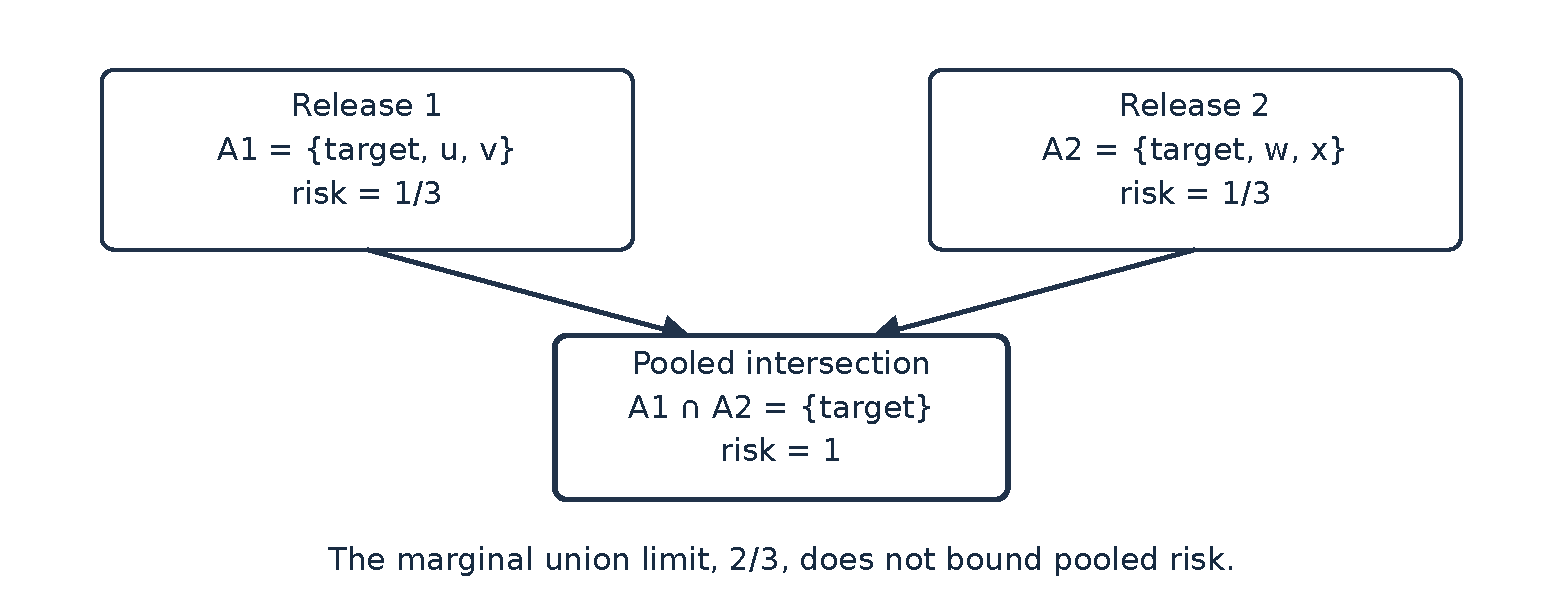
\includegraphics[width=.95\linewidth]{../diagrams/pooling.pdf}
\caption{Two releases that each leave three candidates for the target. Their intersection through the persistent pseudonym leaves one, so the pooled risk is one while the bound~\eqref{eq:union} on single-release success is two thirds.}\label{fig:pool}
\end{figure}

Figure~\ref{fig:pool} shows the smallest case. Each release leaves the target among three candidates, so each alone names the target with probability one third, and the sum of the two single-release risks is two thirds. The two candidate sets share only the target's pseudonym, so the pooled attack names it with certainty. Neither the phenomenon nor the construction is new: complementary and sequential releases that are each $k$-anonymous can be joined to re-identify people \cite{sweeney2002,wang2006,xiao2007}, independently protected releases can be composed into an attack \cite{ganta2008}, and many accurate answers permit reconstruction \cite{dinur2003}. We state it to fix the estimand: a pooled attack that the policy wishes to bound must be registered as a coordinate of its own, because no function of the per-release risks bounds it.

With a persistent pseudonym, releases that publish different projections of the quasi-identifiers can be joined into one table keyed on their union, so Proposition~\ref{prop:pool} says that the programme is one finer release. That suggests rotating the pseudonym between vintages as a cheaper remedy than any audit. It does not help when a published value that identifies the unit stays the same: on the register of Section~\ref{sec:credit}, with exposure published exactly, the pair of key and exposure is unique for every released loan, so each loan can be relinked across vintages from published fields alone. Publishing exposure to one significant figure leaves 10 per cent of loans unique in the first release, so rotation would then remove most of that route; small fresh noise in each vintage would not, since probabilistic record linkage copes with it. Rotation controls linkability; it is not pseudonymisation in the legal sense, which concerns keeping the key that re-identifies units apart \cite{gdpr2016}, and pseudonyms should be keyed so that they cannot be reversed by trying every identifier.

\subsection{From a risk vector to a decision}\label{sec:decision}
A policy declares, for each candidate release, a finite set of coordinates with tolerances $\tau_i$. Let $\alpha\in(0,1)$ be the familywise error level the agency accepts. If $B$ attacks on fresh targets produce $Y$ successes, the exact one-sided Clopper--Pearson upper bound at level $\lambda$ is
\begin{equation}\label{eq:cp}
\overline{R}(Y,B;\lambda)=\begin{cases}1,&Y=B,\\F^{-1}_{\mathrm{Beta}(Y+1,B-Y)}(1-\lambda),&Y<B,\end{cases}
\end{equation}
with $\overline{R}=1-\lambda^{1/B}$ when $Y=0$. For a family of $M$ coordinates fixed before any outcome is seen, $\lambda=\alpha/M$ and a union bound \cite{dunn1961} give simultaneous coverage without assuming the audits are independent. The \emph{audited margin} of coordinate $i$ is then $z_i=1-\overline{R}_i/\tau_i$, and a release is eligible within the declared family when $\min_iz_i\ge0$. That argument fails once the agency reads the audit, adds a coordinate and audits again at the same nominal level: the family is no longer fixed, a problem that also arises for inference after a model is chosen from the data \cite{berk2013}. The gate of Section~\ref{sec:gate} covers that case. It yields a binary decision, not an upper bound; to report an audited margin after adaptive registration, $\overline{R}_i$ must come from a time-uniform confidence sequence \cite{howard2021,waudby2024} with a registered share of the error budget.
